%==============================================================
%  Figura 8.13 - Dispositivo combinato di avvio/arresto con
%  dispositivo di arresto di emergenza (Esempio 6)
%  Adattamento in italiano della Figura 8.13 dell'IFA Report 2/2017
%
%  I simboli riproducono quelli dell'originale: le coordinate sono
%  ricavate dal disegno di partenza (1 cm = 70 px, origine
%  nell'angolo in alto a sinistra della cornice). Nessun cambio di
%  corpo del font: le etichette sono ingrandite con "scale" (vedere
%  la nota nella Figura 8.3).
%==============================================================
\definecolor{verdepotenza}{RGB}{22,67,38}
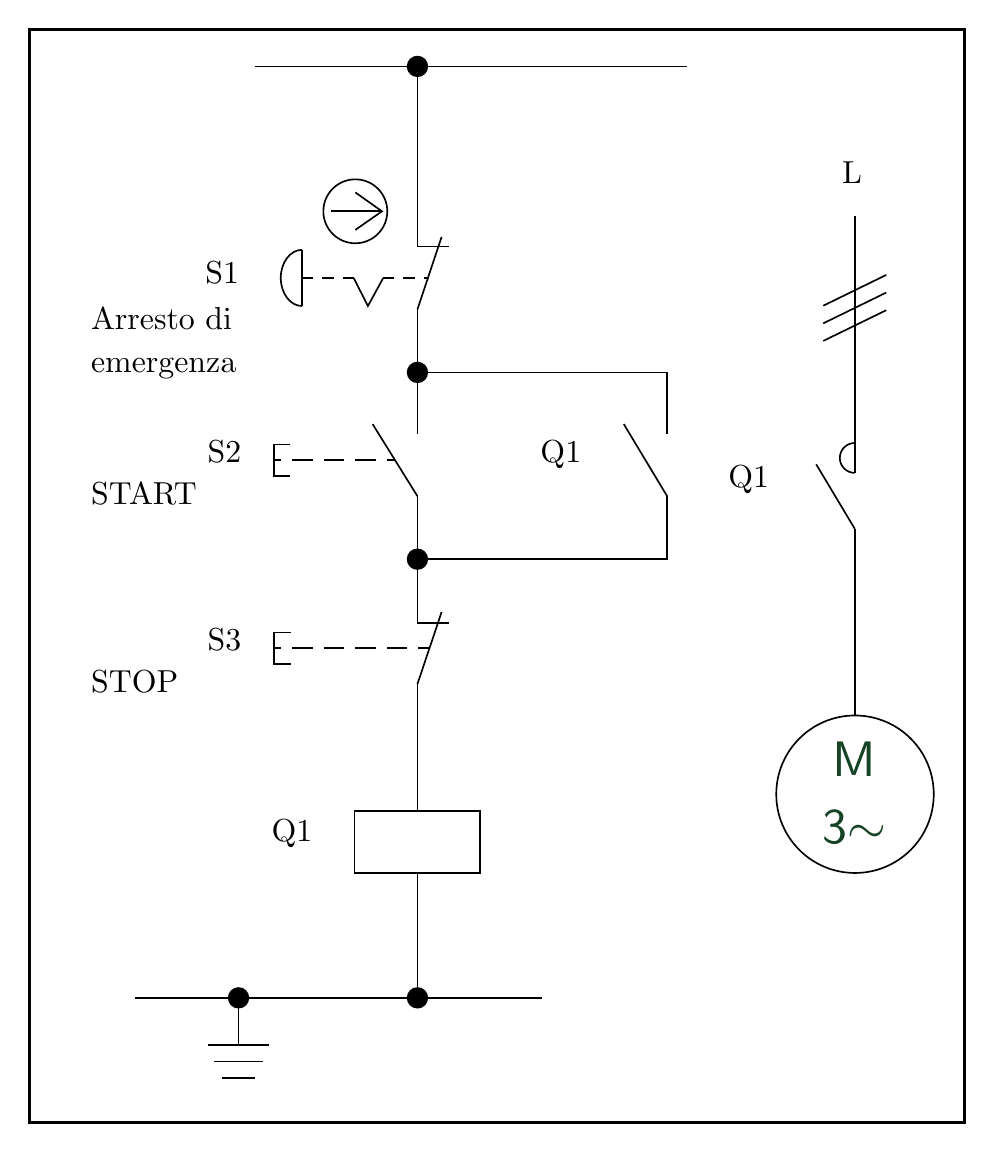
\begin{tikzpicture}[
  font=\normalsize,
  filo/.style={draw=black, line width=0.6pt},
  meccanico/.style={draw=black, line width=0.6pt, dash pattern=on 0.264cm off 0.136cm},
  meccanicocorto/.style={draw=black, line width=0.6pt, dash pattern=on 0.143cm off 0.114cm},
  etichetta/.style={inner sep=1pt, scale=1.15},
  nodo/.style={circle, fill=black, inner sep=0pt, minimum size=0.271cm}
]

%--------------------------------------------------------------
% Cornice
%--------------------------------------------------------------
\draw[draw=black, line width=1.2pt] (0.000,-0.000) rectangle (11.879,-13.879);

%--------------------------------------------------------------
% Linea di alimentazione superiore
%--------------------------------------------------------------
\draw[filo] (2.864,-0.471) -- (8.350,-0.471);
\draw[filo] (4.929,-0.471) -- (4.929,-2.757);
\node[nodo] at (4.929,-0.471) {};

%--------------------------------------------------------------
% S1: dispositivo di arresto di emergenza (pulsante a fungo con
% ritenuta, contatto di apertura ad azionamento meccanico positivo)
%--------------------------------------------------------------
% simbolo di apertura positiva
\draw[filo] (4.140,-2.311) circle (0.406);
\draw[filo] (3.826,-2.311) -- (4.479,-2.311);
\draw[filo] (4.140,-2.071) -- (4.479,-2.311) -- (4.140,-2.547);
% pulsante a fungo
\draw[filo] (3.464,-2.800) -- (3.464,-3.514);
\draw[filo] (3.464,-2.800) arc[start angle=90, end angle=270, x radius=0.271, y radius=0.357];
% collegamento meccanico con ritenuta
\draw[meccanicocorto] (3.464,-3.161) -- (4.121,-3.161);
\draw[filo] (4.121,-3.161) -- (4.300,-3.514) -- (4.493,-3.161);
\draw[meccanicocorto] (4.493,-3.161) -- (5.079,-3.161);
% contatto di apertura
\draw[filo] (4.929,-2.757) -- (5.336,-2.757);
\draw[filo] (4.929,-3.557) -- (5.236,-2.636);
\draw[filo] (4.929,-3.557) -- (4.929,-5.143);
\node[etichetta] at (2.450,-3.086) {S1};
\node[etichetta, anchor=base west] at (0.736,-3.814) {Arresto di};
\node[etichetta, anchor=base west] at (0.736,-4.357) {emergenza};

%--------------------------------------------------------------
% S2: pulsante di START (contatto di chiusura) in parallelo al
% contatto di autoritenuta di Q1
%--------------------------------------------------------------
\node[nodo] at (4.929,-4.357) {};
\draw[filo] (4.929,-4.357) -- (8.100,-4.357) -- (8.100,-5.143);
% pulsante
\draw[filo] (3.311,-5.271) -- (3.111,-5.271) -- (3.111,-5.671) -- (3.311,-5.671);
\draw[filo] (3.111,-5.471) -- (3.193,-5.471);
\draw[meccanico] (3.336,-5.471) -- (4.650,-5.471);
% contatto di chiusura
\draw[filo] (4.929,-5.929) -- (4.360,-5.014);
\draw[filo] (4.929,-5.929) -- (4.929,-7.536);
\node[etichetta] at (2.479,-5.357) {S2};
\node[etichetta, anchor=west] at (0.736,-5.900) {START};
% contatto di autoritenuta Q1
\draw[filo] (8.100,-5.929) -- (7.550,-5.014);
\draw[filo] (8.100,-5.929) -- (8.100,-6.729) -- (4.929,-6.729);
\node[nodo] at (4.929,-6.729) {};
\node[etichetta] at (6.750,-5.400) {Q1};

%--------------------------------------------------------------
% S3: pulsante di STOP (contatto di apertura)
%--------------------------------------------------------------
\draw[filo] (3.319,-7.661) -- (3.111,-7.661) -- (3.111,-8.061) -- (3.319,-8.061);
\draw[filo] (3.111,-7.861) -- (3.193,-7.861);
\draw[meccanico] (3.336,-7.861) -- (5.086,-7.861);
\draw[filo] (4.929,-7.536) -- (5.336,-7.536);
\draw[filo] (4.929,-8.314) -- (5.236,-7.400);
\draw[filo] (4.929,-8.314) -- (4.929,-9.929);
\node[etichetta] at (2.479,-7.757) {S3};
\node[etichetta, anchor=west] at (0.736,-8.286) {STOP};

%--------------------------------------------------------------
% Q1: bobina del contattore, linea di ritorno e messa a terra
%--------------------------------------------------------------
\draw[filo] (4.129,-9.929) rectangle (5.721,-10.714);
\draw[filo] (4.929,-10.714) -- (4.929,-12.300);
\node[etichetta] at (3.336,-10.214) {Q1};
\draw[filo] (1.336,-12.300) -- (6.507,-12.300);
\node[nodo] at (4.929,-12.300) {};
\node[nodo] at (2.657,-12.300) {};
\draw[filo] (2.657,-12.300) -- (2.657,-12.900);
\draw[filo] (2.264,-12.900) -- (3.050,-12.900);
\draw[filo] (2.350,-13.107) -- (2.964,-13.107);
\draw[filo] (2.450,-13.314) -- (2.864,-13.314);

%--------------------------------------------------------------
% Circuito di potenza: linea trifase L, contatto principale di Q1
% e motore M
%--------------------------------------------------------------
\draw[filo] (10.483,-2.371) -- (10.483,-5.633);
\draw[filo] (10.083,-3.510) -- (10.883,-3.119);
\draw[filo] (10.083,-3.734) -- (10.883,-3.343);
\draw[filo] (10.083,-3.957) -- (10.883,-3.567);
\node[etichetta] at (10.450,-1.814) {L};
% contatto principale con apertura automatica
\draw[filo] (10.483,-5.253) arc[start angle=90, end angle=270, radius=0.190];
\draw[filo] (9.993,-5.524) -- (10.483,-6.343);
\draw[filo] (10.483,-6.343) -- (10.483,-8.714);
\node[etichetta] at (9.136,-5.714) {Q1};
% motore trifase
\draw[filo] (10.486,-9.714) circle (1.000);
\node[inner sep=1pt, scale=1.8, text=verdepotenza, font=\sffamily] at (10.479,-9.271) {M};
\node[inner sep=1pt, scale=1.8, text=verdepotenza, font=\sffamily] at (10.479,-10.129) {3$\sim$};

\end{tikzpicture}
